% Aberdeen style guide should be followed when using this
% layout. Their template powerpoint slide is used to extract the
% Aberdeen color and logo but is otherwise ignored (it has little or
% no formatting in it anyway).
%
% http://www.abdn.ac.uk/documents/style-guide.pdf

%%%%%%%%%%%%%%%%%%%% Document Class Settings %%%%%%%%%%%%%%%%%%%%%%%%%
% Pick if you want slides, or draft slides (no animations)
%%%%%%%%%%%%%%%%%%%%%%%%%%%%%%%%%%%%%%%%%%%%%%%%%%%%%%%%%%%%%%%%%%%%%%
%Normal document mode%
%\documentclass[10pt,compress]{beamer}
%Draft or handout mode
\documentclass[10pt,compress,handout]{beamer}
%\documentclass[10pt,compress,handout,ignorenonframetext]{beamer}

%%%%%%%%%%%%%%%%%%%% General Document settings %%%%%%%%%%%%%%%%%%%%%%%
% These settings must be set for each presentation
%%%%%%%%%%%%%%%%%%%%%%%%%%%%%%%%%%%%%%%%%%%%%%%%%%%%%%%%%%%%%%%%%%%%%%
\newcommand{\shortname}{jefferson.gomes@abdn.ac.uk}
\newcommand{\fullname}{Dr Jeff Gomes}
\institute{School of Engineering}
\newcommand{\emailaddress}{}%jefferson.gomes@abdn.ac.uk}
\newcommand{\logoimage}{../FigBanner/UoAHorizBanner}
\title{EX3030/EM40JK}
\subtitle{Transient Heat Transfer}
%\subtitle{Module 1.1: Review of Thermodynamics}
\date[ ]{ }

%%%%%%%%%%%%%%%%%%%% Template settings %%%%%%%%%%%%%%%%%%%%%%%%%%%%%%%
% You shouldn't have to change below this line, unless you want to.
%%%%%%%%%%%%%%%%%%%%%%%%%%%%%%%%%%%%%%%%%%%%%%%%%%%%%%%%%%%%%%%%%%%%%%
\usecolortheme{whale}
\useoutertheme{infolines}

% Use the fading effect for items that are covered on the current
% slide.
\beamertemplatetransparentcovered

% We abuse the author command to place all of the slide information on
% the title page.
\author[\shortname]{%
  \fullname\\\ttfamily{\emailaddress}
}


%At the start of every section, put a slide indicating the contents of the current section.
\AtBeginSection[] {
  \begin{frame}
    \frametitle{Section Outline}
    \tableofcontents[currentsection]
  \end{frame}
}

% Allow the inclusion of movies into the Presentation! At present,
% only the Okular program is capable of playing the movies *IN* the
% presentation.
\usepackage{multimedia}
\usepackage{animate}

%% Handsout -- comment out the lines below to create handstout with 4 slides in a page with space for comments
\usepackage{handoutWithNotes}

\mode<handout>
{
\usepackage{pgf,pgfpages}

\pgfpagesdeclarelayout{2 on 1 boxed with notes}
{
\edef\pgfpageoptionheight{\the\paperheight} 
\edef\pgfpageoptionwidth{\the\paperwidth}
\edef\pgfpageoptionborder{0pt}
}
{
\setkeys{pgfpagesuselayoutoption}{landscape}
\pgfpagesphysicalpageoptions
    {%
        logical pages=4,%
        physical height=\pgfpageoptionheight,%
        physical width=\pgfpageoptionwidth,%
        last logical shipout=2%
    } 
\pgfpageslogicalpageoptions{1}
    {%
    border code=\pgfsetlinewidth{1pt}\pgfstroke,%
    scale=1,
    center=\pgfpoint{.25\pgfphysicalwidth}{.75\pgfphysicalheight}%
    }%
\pgfpageslogicalpageoptions{2}
    {%
    border code=\pgfsetlinewidth{1pt}\pgfstroke,%
    scale=1,
    center=\pgfpoint{.25\pgfphysicalwidth}{.25\pgfphysicalheight}%
    }%
\pgfpageslogicalpageoptions{3}
    {%
    border shrink=\pgfpageoptionborder,%
    resized width=.7\pgfphysicalwidth,%
    resized height=.5\pgfphysicalheight,%
    center=\pgfpoint{.75\pgfphysicalwidth}{.29\pgfphysicalheight},%
    copy from=3
    }%
\pgfpageslogicalpageoptions{4}
    {%
    border shrink=\pgfpageoptionborder,%
    resized width=.7\pgfphysicalwidth,%
    resized height=.5\pgfphysicalheight,%
    center=\pgfpoint{.75\pgfphysicalwidth}{.79\pgfphysicalheight},%
    copy from=4
    }%

\AtBeginDocument
    {
    \newbox\notesbox
    \setbox\notesbox=\vbox
        {
            \hsize=\paperwidth
            \vskip-1in\hskip-1in\vbox
            {
                \vskip1cm
                Notes\vskip1cm
                        \hrule width\paperwidth\vskip1cm
                    \hrule width\paperwidth\vskip1cm
                        \hrule width\paperwidth\vskip1cm
                    \hrule width\paperwidth\vskip1cm
                        \hrule width\paperwidth\vskip1cm
                    \hrule width\paperwidth\vskip1cm
                    \hrule width\paperwidth\vskip1cm
                    \hrule width\paperwidth\vskip1cm
                        \hrule width\paperwidth
            }
        }
        \pgfpagesshipoutlogicalpage{3}\copy\notesbox
        \pgfpagesshipoutlogicalpage{4}\copy\notesbox
    }
}
}

%\pgfpagesuselayout{2 on 1 boxed with notes}[letterpaper,border shrink=5mm]
%\pgfpagesuselayout{2 on 1 boxed with notes}[letterpaper,border shrink=5mm]



%%%%% Color settings
\usepackage{color}
%% The background color for code listings (i.e. example programs)
\definecolor{lbcolor}{rgb}{0.9,0.9,0.9}%
\definecolor{UoARed}{rgb}{0.64706, 0.0, 0.12941}
\definecolor{UoALight}{rgb}{0.85, 0.85, 0.85}
\definecolor{UoALighter}{rgb}{0.92, 0.92, 0.92}
\setbeamercolor{structure}{fg=UoARed} % General background and higlight color
\setbeamercolor{frametitle}{bg=black} % General color
\setbeamercolor{frametitle right}{bg=black} % General color
\setbeamercolor{block body}{bg=UoALighter} % For blocks
\setbeamercolor{structure}{bg=UoALight} % For blocks
% Rounded boxes for blocks
\setbeamertemplate{blocks}[rounded]

%%%%% Font settings
% Aberdeen requires the use of Arial in slides. We can use the
% Helvetica font as its widely available like so
% \usepackage{helvet}
% \renewcommand{\familydefault}{\sfdefault}
% But beamer already uses a sans font, so we will stick with that.

% The size of the font used for the code listings.
\newcommand{\goodsize}{\fontsize{6}{7}\selectfont}

% Extra math packages, symbols and colors. If you're using Latex you
% must be using it for formatting the math!
\usepackage{amscd,amssymb} \usepackage{amsfonts}
\usepackage[mathscr]{eucal} \usepackage{mathrsfs}
\usepackage{latexsym} \usepackage{amsmath} \usepackage{bm}
\usepackage{amsthm} \usepackage{textcomp} \usepackage{eurosym}
% This package provides \cancel{a} and \cancelto{a}{b} to "cancel"
% expressions in math.
\usepackage{cancel}

\usepackage{comment} 

% Get rid of font warnings as modern LaTaX installations have scalable
% fonts
\usepackage{type1cm} 

%\usepackage{enumitem} % continuous numbering throughout enumerate commands

% For exact placement of images/text on the cover page
\usepackage[absolute]{textpos}
\setlength{\TPHorizModule}{1mm}%sets the textpos unit
\setlength{\TPVertModule}{\TPHorizModule} 

% Source code formatting package
\usepackage{listings}%
\lstset{ backgroundcolor=\color{lbcolor}, tabsize=4,
  numberstyle=\tiny, rulecolor=, language=C++, basicstyle=\goodsize,
  upquote=true, aboveskip={1.5\baselineskip}, columns=fixed,
  showstringspaces=false, extendedchars=true, breaklines=false,
  prebreak = \raisebox{0ex}[0ex][0ex]{\ensuremath{\hookleftarrow}},
  frame=single, showtabs=false, showspaces=false,
  showstringspaces=false, identifierstyle=\ttfamily,
  keywordstyle=\color[rgb]{0,0,1},
  commentstyle=\color[rgb]{0.133,0.545,0.133},
  stringstyle=\color[rgb]{0.627,0.126,0.941}}

% Allows the inclusion of other PDF's into the final PDF. Great for
% attaching tutorial sheets etc.
\usepackage{pdfpages}
\setbeamercolor{background canvas}{bg=}  

% Remove foot note horizontal rules, they occupy too much space on the slide
\renewcommand{\footnoterule}{}

% Force the driver to fix the colors on PDF's which include mixed
% colorspaces and transparency.
\pdfpageattr {/Group << /S /Transparency /I true /CS /DeviceRGB>>}

% Include a graphics, reserve space for it but
% show it on the next frame.
% Parameters:
% #1 Which slide you want it on
% #2 Previous slides
% #3 Options to \includegraphics (optional)
% #4 Name of graphic
\newcommand{\reserveandshow}[4]{%
\phantom{\includegraphics<#2|handout:0>[#3]{#4}}%
\includegraphics<#1>[#3]{#4}%
}
\usepackage{xcolor}

\newlength{\overwritelength}
\newlength{\minimumoverwritelength}
\setlength{\minimumoverwritelength}{1cm}
\newcommand{\overwrite}[3][red]{%
  \settowidth{\overwritelength}{$#2$}%
  \ifdim\overwritelength<\minimumoverwritelength%
    \setlength{\overwritelength}{\minimumoverwritelength}\fi%
  \stackrel
    {%
      \begin{minipage}{\overwritelength}%
        \color{#1}\centering\small #3\\%
        \rule{1pt}{9pt}%
      \end{minipage}}
    {\colorbox{#1!50}{\color{black}$\displaystyle#2$}}} 

\newcommand{\frc}{\displaystyle\frac}
\newcommand{\red}{\textcolor{red}}
\newcommand{\blue}{\textcolor{blue}}
\newcommand{\green}{\textcolor{green}}
\newcommand{\purple}{\textcolor{purple}} 

\begin{document}

% Title page layout
\begin{frame}
  \titlepage
  \vfill%
  \begin{center}
    \includegraphics[clip,width=0.8\textwidth]{\logoimage}
  \end{center}
\end{frame}

% Table of contents
%\frame{ \frametitle{Slides Outline}
%  \tableofcontents
%}


%%%%%%%%%%%%%%%%%%%% The Presentation Proper %%%%%%%%%%%%%%%%%%%%%%%%%
% Fill below this line with \begin{frame} commands! It's best to
% always add the fragile option incase you're going to use the
% verbatim environment.
%%%%%%%%%%%%%%%%%%%%%%%%%%%%%%%%%%%%%%%%%%%%%%%%%%%%%%%%%%%%%%%%%%%%%%

%%%
%%% SECTION
%%%
\section{Introduction} 


%%% SUBSECTION
\subsection{Objectives}

%%%
%%% Slide
%%%
\begin{frame}
 \frametitle{Aims and Objectives}
   \begin{enumerate}
     \item<1-> In previous lectures, the main focus was on methods to calculate heat transfer flux under steady-state conditions;
     \item<1-> However, several environmental and industrial applications require understanding of transient (or unsteady) heat transfer mechanisms;
     \item<2-> In this module we will study two main heat transfer scenarios,
         \begin{enumerate}
            \item<2-> The simplest case when the spatial variation of temperature is negligible, and temperature varies nearly uniformly with time ({\it lumped capacity method}) -- $T=T\left(t\right)$;
            \item<3-> The most common case is when temperature varies in space and time -- $T=T\left(x, t\right)$;
            \item<3-> For this, we will study two classes of methods, analytical and numerical methods for 1D. 
         \end{enumerate}
   \end{enumerate}
\end{frame}


%%%
%%% SUBSECTION
%%%
\subsection{Bibliography} 

%%%
%%% Slide
%%%
\begin{frame}
 \frametitle{Suggested References}
  Literature relevant for this module:
  \begin{enumerate}[{[}1{]}]
    \item J.P. Holman, `Heat Transfer', 10$^{th}$ Edition (McGraw-Hill): Chapter 4;
    \item F.P. Incropera, D.P. DeWitt, T.L.Bergman, A.S. Lavine, `Introduction to Heat Transfer' (John Willey $\&$ Sons): Chapters 5;
    \item Y.A. Cengel, `Heat Transfer: A Practical Approach', 2$^{nd}$ Edition (McGraw-Hill): Chapters 4 and 5;
    \item L. Theodore, `Essential Engineering Calculations Series: Heat Transfer Applications for the Practicing Engineer' (John Willey $\&$ Sons): Chapter 8.
  \end{enumerate}
\end{frame}
 

%%%
%%%  SECTION
%%%
\section{Lumped-Capacity Method}
%\section{Unsteady-State Conduction}

%%% SUBSECTION
\subsection{Introduction}

%%%
%%% Slide
%%%
\begin{frame}
 \frametitle{Introduction}
   \begin{columns}
     \begin{column}[l]{0.5\linewidth}
        \begin{center}
          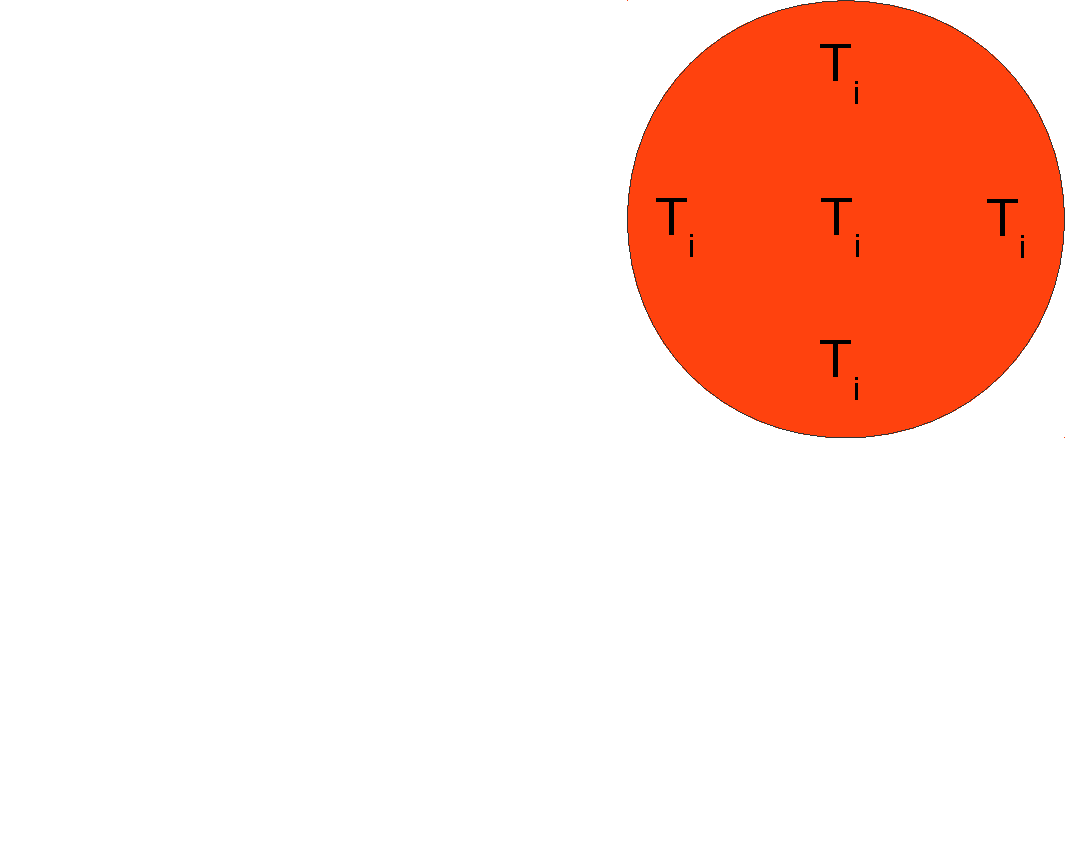
\includegraphics[width=\columnwidth,clip]{./Pics/Lumped1}
        \end{center}
     \end{column}
%
     \begin{column}[l]{0.5\linewidth}
        \begin{enumerate}
           \item<1-> In the study of heat transfer, the simplest case analysis is when bodies are assumed {\it isothermal} and, therefore they can be treated as a \blue{lump} system;
           \item<1-> This means that the temperature of these bodies at any spatial coordinate can be expressed as function of time only, i.e., \blue{$T=T\left(t\right)$};
        \end{enumerate}
     \end{column}     
   \end{columns}
\end{frame}

%%%
%%% SUBSECTION
%%%
\subsection{Thermal Energy Balance}

%%%
%%% Slide
%%%
\begin{frame}
 \frametitle{Thermal Energy Balance}
   \begin{enumerate}
     \item<1-> Let's consider a body of mass \blue{$m$} and arbitrary shape $\left(\text{with area} \blue{A_{s}}\right)$ and temperature \blue{$T$};
     \item<1-> The body is assumed homogeneous and we can consider constant heat capacity at constant pressure, \blue{$C_{p}$}, thermal conductivity, \blue{$\kappa$} and;
     \item<2-> The energy balance of an isothermal body during time interval \blue{$dt$}, subject to constant surrounding temperature \blue{$T_{\infty}$}, can be simplified as,\\
       \begin{center}
        \begin{tabular}{c c c}
           \visible<3->{\blue{Heat transferred into}} & \visible<3->{=} & \visible<4->{\red{Increase of thermal energy}} \\
           \visible<3->{\blue{the body during $dt$}}  &                 & \visible<4->{\red{of the body during $dt$}} \\
                                                      &                 & \\
           \visible<3->{\blue{$\Downarrow$}}          &                 & \visible<4->{\red{$\Downarrow$}}\\
                                                      &                 & \\
           \visible<3->{\blue{$hA_{s}\left(T_{\infty}-T\right)dt$}}& \visible<3->{=} & \visible<4->{\red{$mC_{p}dT$}}
        \end{tabular}
        \end{center} 
      \item<5-> For \blue{$m=\rho V$} (where $\rho$ and $V$ are the density and volume of the body, respectively) and;
      \item<5-> \blue{$dT=d\left(T_{\infty}-T\right)$};
   \end{enumerate}
\end{frame}

%%%
%%% Slide
%%%
\begin{frame}
 \frametitle{Thermal Energy Balance}
   \begin{enumerate}\setcounter{enumi}{5}\scriptsize
     \item<1-> The energy balance,
          \visible<1->{\blue{\begin{equation}
              hA_{s}\left(T_{\infty}-T\right)dt = mC_{p}dT \label{eqn:energybalance}
          \end{equation}}}
     \item<1-> can be rearranged and integrated as (from time \blue{0} to \blue{t}),
          \visible<2->{\begin{eqnarray}
              \frc{d\left(T-T_{\infty}\right)}{T-T_{\infty}} &=& -\frc{hA_{s}}{\rho V C_{p}}dt \nonumber \\
              \ln\frc{T(t)-T_{\infty}}{T_{0}-T_{\infty}} &=& -\frc{hA_{s}}{\rho V C_{p}}t \nonumber \\
              \blue{\frc{T(t)-T_{\infty}}{T_{0}-T_{\infty}}} &\blue{=}& \blue{e^{-bt}} \label{eqn:CharacteristicTime}
          \end{eqnarray}}
          \visible<2->{where \blue{$T_{0}$} is the initial temperature and $b = \frc{hA_{s}}{\rho V C_{p}}$ is the \blue{time constant} with dimension {\bf $\left[\text{time}^{-1}\right]$}.}
     \item<3-> From Eqn.~\ref{eqn:CharacteristicTime}:
        \begin{enumerate}\scriptsize
           \item<3-> We can calculate either the temperature \blue{$T(t)$} of the body at a given time \blue{$t$} or;
           \item<4-> The time \blue{$t$} required for a body to reach temperature \blue{$T(t)$};
           \item<5-> Temperature \blue{$T(t)$} approaches the surrounding temperature \blue{$T_{\infty}$} {\bf exponentially};
           \item<6-> A large value of \blue{b} indicates a higher rate of temperature decay;
           \item<7-> Finally, \blue{b} is proportional to \blue{$A_{s}$} and inversely proportional to \blue{$m$} and \blue{$C_{p}$} of the body. This means that it takes longer to heat or cool a larger mass, in particular if it also has a large heat capacity.
        \end{enumerate}
   \end{enumerate}
\end{frame}


%%%
%%% SUBSECTION
%%%
\subsection{Convection Heat Transfer}

%%%
%%% Slide
%%%
\begin{frame}
 \frametitle{Convection Heat Transfer}
   \begin{enumerate}%\setcounter{enumi}{5}\scriptsize
     \item<1-> The {\it Newton's law of cooling} can determine the rate of convection heat transfer,
          \visible<1->{\blue{\begin{equation}
              \dot{Q}(t) = hA_{s}\left[T(t) - T_{\infty}\right] \hspace{1cm} \mathbf{(W)}
          \end{equation}}}
     \item<2-> The heat transferred between the body and the surroundings during time \blue{$\Delta t$} is the energy change in the system (i.e., body + surroundings):
          \visible<2->{\begin{equation}
              \dot{Q} = m C_{p}\left[T(t) - T_{\infty}\right] \hspace{1cm} \mathbf{(J)}
          \end{equation}}
     \item<3-> Therefore the maximum heat exchanged between the body and the surroundings is
          \visible<3->{\begin{equation}
              \dot{Q}_{\text{max}} = m C_{p}\left[T_{0} - T_{\infty}\right] \hspace{1cm} \mathbf{(J)}
          \end{equation}}
   \end{enumerate}
\end{frame}

%%%
%%% SUBSECTION
%%%
\subsection{Criteria for Lumped System}


%%%
%%% Slide
%%%
\begin{frame}
 \frametitle{Criteria for Lumped System}
   \begin{enumerate}%\setcounter{enumi}{5}\scriptsize
     \item<1-> The assumption of {\bf lumped system} is not often the most appropriate. With the {\it characteristic length} \blue{$L_{c}=\frc{V}{A_{s}}$};
     \item<2-> We can determine the dimensionless \red{Biot Number (\it{Bi})},
       \begin{equation}
          \visible<2->{\red{Bi} \blue{= \frc{\text{Conduction resistance within the body}}{\text{Convection resistance at the surface}}}} \visible<3->{\blue{= \frc{\frc{L_{c}}{\kappa}}{\frc{1}{h}}} \red{= \frc{h L_{c}}{\kappa}}}
       \end{equation}  
     \item<4-> {\bf Lumped system} analysis assumes {\it uniform temperature distribution} throughout the body;
     \item<4-> This assumption is correct {\bf if} the convection coefficient is small and thermal conductivity is large, i.e.,;
     \item<5-> \blue{The smaller the {\bf Bi}, the more accurate the lumped system analysis,} 
                     \begin{displaymath}
                       \visible<5->{ \red{Bi \leq 0.1}}
                     \end{displaymath}
   \end{enumerate}
\end{frame}

%%%
%%% Slide
%%%
\begin{frame}
 \frametitle{Criteria for Lumped System -- Example 1}
   \begin{enumerate}%\scriptsize
     \item<1-> Example: Two spheres are removed from a furnace and let to cool with air at 25$^{\circ}$C under relatively low convection coefficient of 15 W.$\left(\text{m}^{2}.^{\circ}\text{C}\right)$. The spheres are made of copper,  $\kappa_{\text{Cu}}=401\;\text{W.}\left(\text{m.}^{\circ}\text{C}\right)^{-1}$, and coal, $\kappa_{\text{Coal}}=0.2\;\text{W.}\left(\text{m.}^{\circ}\text{C}\right)^{-1}$. Can we apply the lumped method to both spheres? 
   \end{enumerate}
\end{frame}

%%%
%%% Slide
%%%
\begin{frame}
 \frametitle{Criteria for Lumped System --  Example 2}
   \begin{enumerate}\setcounter{enumi}{1}%\scriptsize % Holman pg 143
      \item A steel ball of 5 cm in diameter and at uniform temperature of 450$^{\circ}$C is suddenly placed in a controlled environment where temperature is kept at 100$^{\circ}$C.  The prescribed convection heat transfer coefficient is 10 W.$\left(\text{m}^{2}.^{\circ}\text{C}\right)^{-1}$. Calculate the time required for the ball to reach 150$^{\circ}$C. \\
Given C$_{p,\text{steel}} = 0.46\text{ kJ.kg}^{-1}$, $\kappa_{\text{steel}}=35\text{ W.}\left(\text{m.}^{\circ}\text{C}\right)$ and $\rho_{\text{steel}}=7.8\times 10^{3}\text{kg.m}^{-3}$.
   \end{enumerate}
\end{frame}


%%%
%%% SECTION
%%%
\section{Transient Heat Conduction in Prescribed Geometries}

%%%
%%% Slide
%%%
\begin{frame}
 \frametitle{Introduction}
   \begin{enumerate}%\setcounter{enumi}{5}%\scriptsize
     \item<1-> In most transient heat transfer problems, the \blue{\it Biot} dimensionless number is larger than \blue{0.1} and the \blue{lumped-capacity method} and Eqn.~\ref{eqn:CharacteristicTime} can not be used.
     \item<2-> In such cases, it is necessary to calculate the temperature distribution throught spatial and time domains, i.e., \red{$T\left(\underline{x},t\right)$}, where $\underline{x}$ is the spatial-coordinate in 1-, 2- and 3-D;
   \end{enumerate}

   \begin{center}
      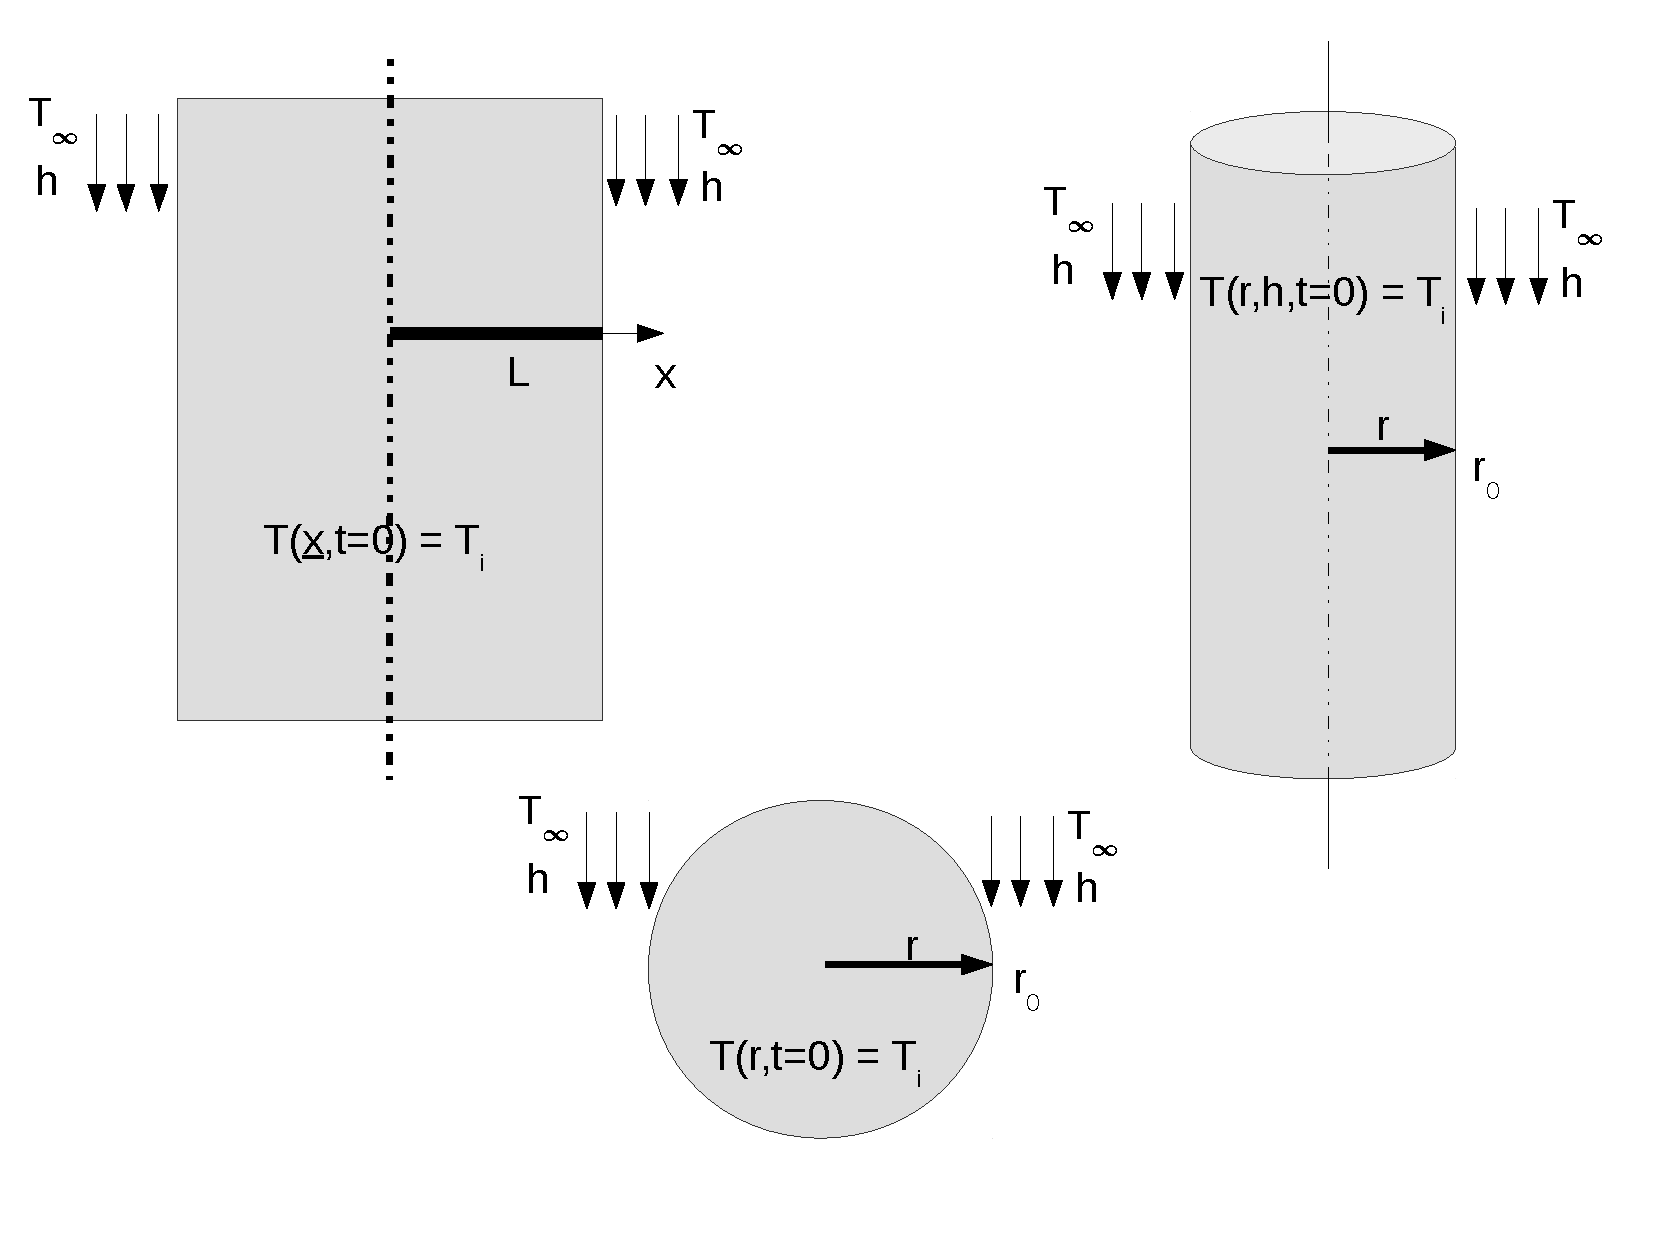
\includegraphics[width=0.55\columnwidth,height=0.45\columnwidth,clip]{./Pics/HT_All}
   \end{center}
\end{frame}


%%%
%%% SUBSECTION
%%%
\subsection{Analytical Methods}

%%%
%%% Slide
%%%
\begin{frame}
 \frametitle{Plane Wall}
  \begin{columns}
    \begin{column}[l]{0.6\linewidth}
     \begin{enumerate}[(a)]%\scriptsize
        \item<1-> Let's assume a plane wall of thickness $2L$ with initial uniform temperature distribution $T\left(\underline{x},t=0\right)=T_{i}$;
        \item<1-> The wall is surrounded by a fluid with constant temperature $T_{\infty}$ imposing a convective heat transfer coefficient $h$;
        \item<1-> Also, let's assume that the wall's height and width are infinite and the problem can be considered as \blue{1-D};
        \item<1-> Finally, all thermo-physical properties are considered constant, and there is no heat generation;  
        \item<1-> If the geometry is uniform, we can assume the axis of symmetry at \blue{$x=0$};
     \end{enumerate}
    \end{column}
     \begin{column}[l]{0.4\linewidth}
        \begin{center}
          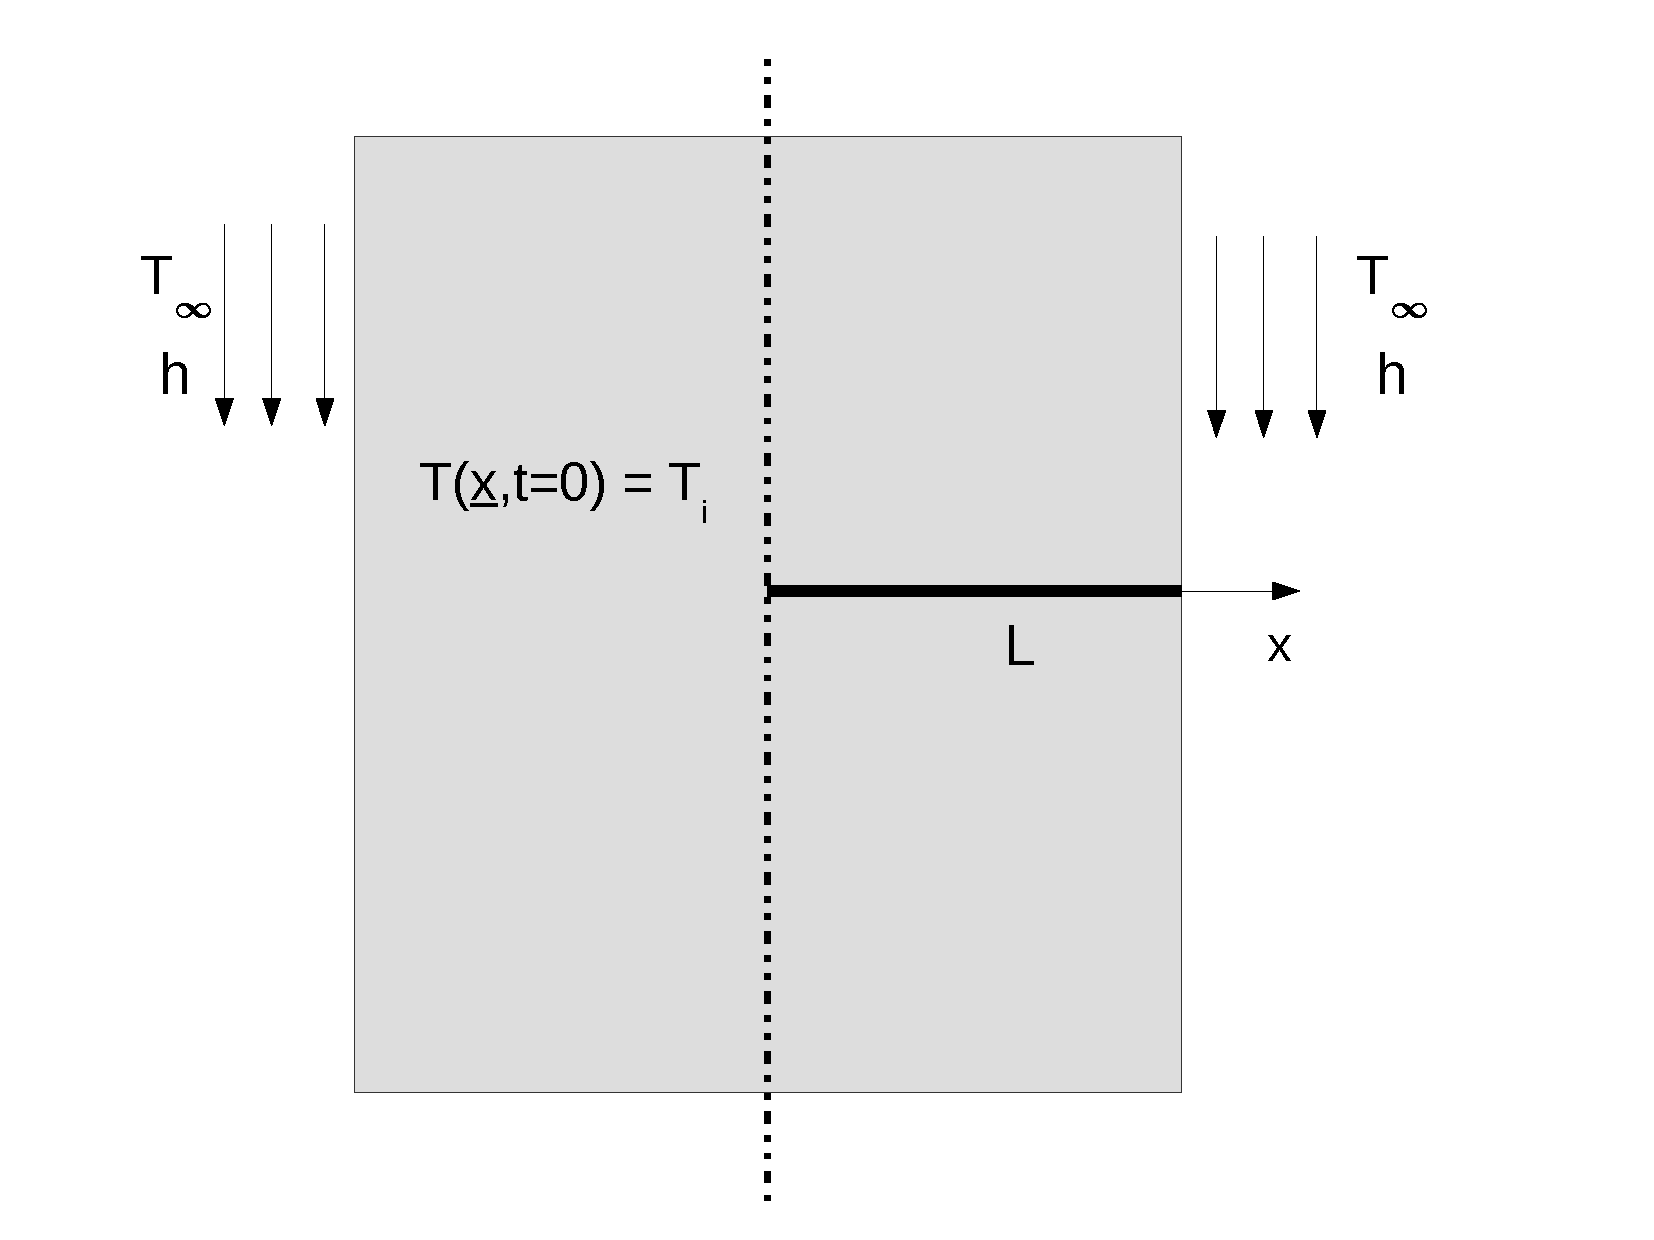
\includegraphics[width=1.1\columnwidth,height=1.3\columnwidth,clip]{./Pics/HT_PlaneWall}
        \end{center}
    \end{column}
  \end{columns}
\end{frame}


%%%
%%% Slide
%%%
\begin{frame}
 \frametitle{Plane Wall: 1-D Transient Heat Conduction at \red{$0\leq x\leq L$} }
  \begin{columns}
    \begin{column}[l]{0.6\linewidth}
      \begin{block}{\begin{center}Heat Equation\end{center}}
           \visible<1->{\begin{equation}
              \frc{\partial^{2} T}{\partial x^{2}} = \frc{1}{\alpha}\frc{\partial T}{\partial t}\label{Eqn:GlobalThermalEqn}
           \end{equation}
        \scriptsize where $\alpha=\kappa\left(\rho C_{p}\right)^{-1}$ is the heat diffusivity of the material.}
      \end{block}

      \visible<2->{\begin{block}{\begin{center}Boundary Conditions\end{center}}
           \begin{eqnarray}
              && \frc{\partial}{\partial x} T\left(x=0,t\right) = 0 \nonumber \\
              && -\kappa \frc{\partial}{\partial x}T\left(x=L,t\right) = h\left[T\left(x=L,t\right) - T_{\infty}\right] \nonumber
           \end{eqnarray}
      \end{block}}

      \visible<3->{\begin{block}{\begin{center}Initial Conditions\end{center}}
           \begin{displaymath}
               T\left(x,t=0\right) = T_{i}
           \end{displaymath}
      \end{block}}

    \end{column}
     \begin{column}[l]{0.4\linewidth}
        \begin{center}
          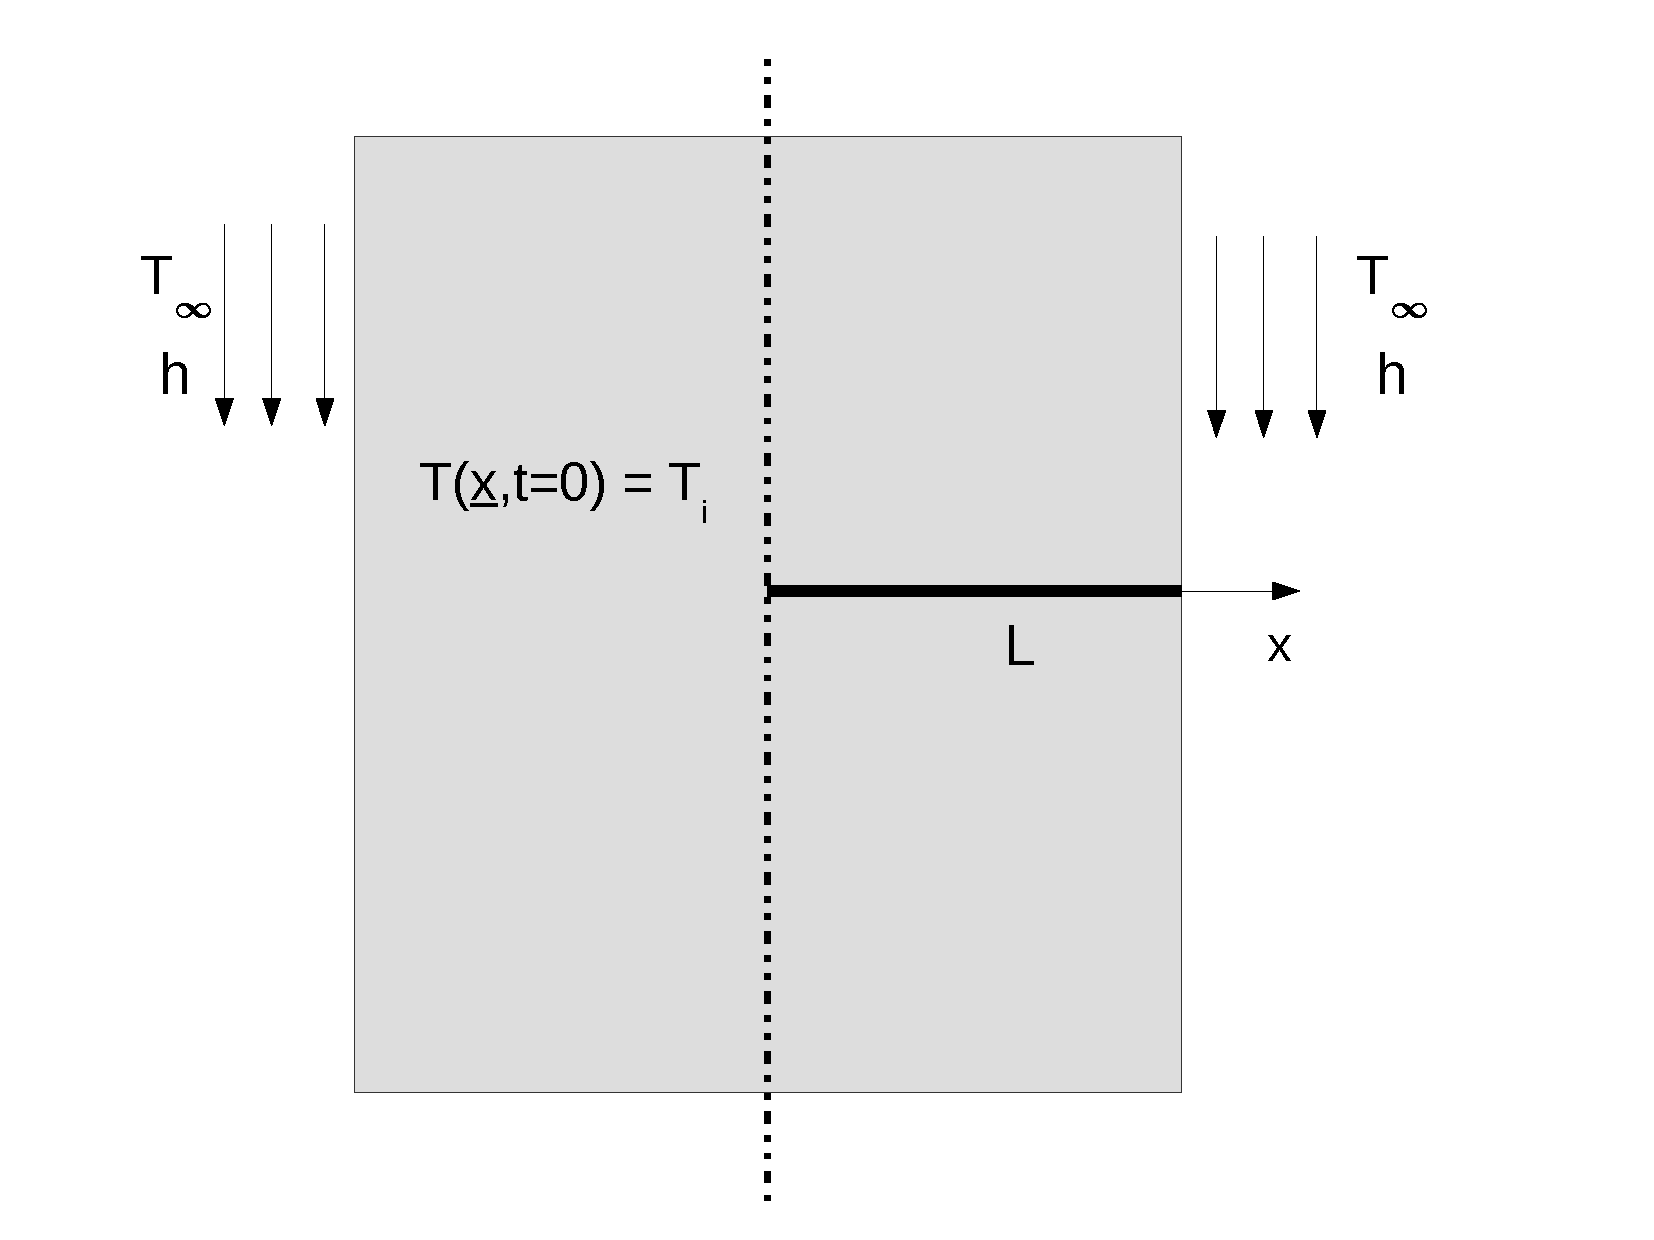
\includegraphics[width=1.1\columnwidth,height=1.3\columnwidth,clip]{./Pics/HT_PlaneWall}
        \end{center}
    \end{column}
  \end{columns}
\end{frame}

%%%
%%% Slide
%%%
\begin{frame}
 \frametitle{Plane Wall: 1-D Transient Heat Conduction at \red{$0\leq x\leq L$} }
   \begin{enumerate}[(a)]\setcounter{enumi}{5}%\scriptsize
     \item<1-> In order to solve Eqn.~\ref{Eqn:GlobalThermalEqn} with the associated boundary and initial conditions, we first need to {\it adimensionalise} this partial differential equation (PDE) with
        \begin{displaymath}
             \theta = \frc{T - T_{\infty}}{T_{i} - T_{\infty}}
        \end{displaymath}    
     \item<2-> Leading to (in non-dimensional form):
           \visible<2->{\begin{equation}
              \frc{\partial^{2} \theta}{\partial X^{2}} = \frc{\partial \theta}{\partial \tau}\label{Eqn:GlobalThermalEqn_NonDimensional}
           \end{equation}
           where $X = x/L$ and $\tau = \alpha t / L^{2}$.}
     \item<3-> With {\it boundary conditions}:
           \visible<3->{\begin{eqnarray}
              \frc{\partial \theta}{\partial X} = 0\;\;\;        &&\text{ at } X=0\text{ and } \tau > 0 \nonumber \\
              \frc{\partial \theta}{\partial X} = -Bi\cdot\theta && \text{ at } X=L \text{ and } \tau > 0 \nonumber
           \end{eqnarray}}
      \item<3-> And {\it initial conditions}:
           \visible<3->{\begin{displaymath}
               \theta\left(X,\tau=0\right) = 1
           \end{displaymath}}
   \end{enumerate} 
\end{frame}


%%%
%%% Slide
%%%
\begin{frame}
 \frametitle{Plane Wall: 1-D Transient Heat Conduction at \red{$0\leq x\leq L$} }
   \begin{enumerate}[(a)]\setcounter{enumi}{9}%\scriptsize
     \item<1-> The solution of Eqn.~\ref{Eqn:GlobalThermalEqn_NonDimensional} involves using Fourier series expansion,
          \visible<1->{\begin{displaymath}
             \theta = \sum\limits_{n=1}^{\infty} A_{n}\exp\left(-\lambda^{2}_{n}\tau\right)\cos{\left(\lambda_{n}X\right)}
          \end{displaymath}}
          with
          \begin{displaymath}
            A_{n} = \frc{4\sin{\lambda_{n}}}{2\lambda_{n}+\sin{2\lambda_{n}}}\text{ and } \lambda_{n}\tan{\lambda_{n}} = Bi
          \end{displaymath}
     \item<2-> The solution for this infinite series converges rapidly with increasing time and for $\tau > 0.2$. We can use the first term and neglect the remaining terms; 
     \item<3-> Solution for $\tau>0.2$ can be found in the next slide for the 3 geometries considered here.

   \end{enumerate} 
\end{frame}


%%%
%%% Slide
%%%
\begin{frame}
 \frametitle{1-D Transient Heat Conduction (with $\tau > 0.2$)}
   \begin{enumerate}[(a)]%\setcounter{enumi}{9}%\scriptsize
     \item<1-> Plane Wall:
        \begin{equation}
           \theta_{\text{wall}} = \frc{T(x,t)-T_{\infty}}{T_{i}-T_{\infty}}= A_{1}e^{-\lambda_{1}^{2}\tau}\cos{\left(\frc{\lambda_{1}x}{L}\right)}\label{analytical:wall}
        \end{equation}
     \item<2-> Cylinder:
        \begin{equation}
           \theta_{\text{cyl}} = \frc{T(r,t)-T_{\infty}}{T_{i}-T_{\infty}}= A_{1}e^{-\lambda_{1}^{2}\tau}\mathbf{J_{0}}\left(\frc{\lambda_{1}r}{r_{0}}\right)\label{analytical:cylinder}
        \end{equation}
     \item<3-> Sphere:
        \begin{equation}
           \theta_{\text{sph}} = \frc{T(r,t)-T_{\infty}}{T_{i}-T_{\infty}}= A_{1}e^{-\lambda_{1}^{2}\tau}\frc{\sin{\left(\frc{\lambda_{1}r}{r_{0}}\right)}}{\frc{\lambda_{1}r}{r_{0}}}\label{analytical:sphere}
        \end{equation}

     \item<4-> At the centre of the geometry: $\cos{0}=1=\mathbf{J_{0}}(0)=1$ and the limit of $\frac{sin{x}}{x}$ is 1.
         \begin{equation}
             \theta_{0,\text{wall}} = \theta_{0,\text{cyl}} = \theta_{0,\text{sph}} = \frc{T_{0}-T_{\infty}}{T_{i}-T_{\infty}} = A_{1}e^{-\lambda_{1}^{2}\tau}
         \end{equation}
   \end{enumerate} 
   \visible<1->{$A_{1}$ and $\lambda_{1}$ are functions of the $Bi$ dimensioneless number. Function $J_{0}$ is the zeroth-order Bessel function of the first kind (see Tables in Appendix 1).}

\end{frame}


%%%
%%% Slide
%%%
\begin{frame}
 \frametitle{Energy Balance}
   \begin{enumerate}[(a)]%\setcounter{enumi}{9}%\scriptsize
     \item<1-> The maximum amount of heat that can be transferred \red{from/to} a body occurs when the temperature of the body changes from the \blue{initial temperature, $T_{i}$} to \red{ambient temperature, $T_{\infty}$},
         \begin{displaymath}
             \visible<1->{\mathcal{Q}_{\text{max}} = m C_{p}\left(T_{\infty}-T_{i}\right)} \visible<2->{= \rho V C_{p}\left(T_{\infty}-T_{i}\right)} 
         \end{displaymath}
     \item<3-> The amount of heat \blue{$\mathcal{Q}$} transferred at a time \blue{$t$} is,
              \visible<3->{\begin{displaymath}
                 \mathcal{Q} = \int\limits_{V} \rho C_{p}\left[T\left(x,t\right)-T_{i}\right]dV
              \end{displaymath}}
     \item<4-> Assuming that $\left(\rho C_{p}\right)$ remains constant,
              \visible<4->{\begin{displaymath}
                 \frc{\mathcal{Q}}{\mathcal{Q}_{\text{max}}} = \frc{\int\limits_{V} \rho C_{p}\left[T\left(x,t\right)-T_{i}\right]dV}{\rho V C_{p}\left(T_{\infty}-T_{i}\right)} = \frc{1}{V}\int\limits_{V}\left(1-\theta\right)dV
              \end{displaymath}}
   \end{enumerate} 
\end{frame}


%%%
%%% Slide
%%%
\begin{frame}
 \frametitle{Energy Balance}
   \begin{enumerate}[(a)]\setcounter{enumi}{3}%\scriptsize
     \item<1-> We can perform the integration for all three  studied geometries:
          \begin{eqnarray}
            \text{Plane wall:} && \left(\frc{\mathcal{Q}}{\mathcal{Q}_{\text{max}}}\right)_{\text{wall}} = 1 - \theta_{0,\text{wall}}\frc{\sin{\lambda_{1}}}{\lambda_{1}} \\
            \text{Cylinder:} && \left(\frc{\mathcal{Q}}{\mathcal{Q}_{\text{max}}}\right)_{\text{cyl}} = 1- 2\theta_{0,\text{cyl}}\frc{\mathbf{J_{1}}}{\lambda_{1}} \\
            \text{Sphere:} && \left(\frc{\mathcal{Q}}{\mathcal{Q}_{\text{max}}}\right)_{\text{sph}} = 1 - 3\theta_{0,\text{sph}}\frc{\sin{\lambda_{1}}-\lambda_{1}\cos{\lambda_{1}}}{\lambda_{1}^{3}}
          \end{eqnarray}
      \item<2-> Heisler and Gr\"ober charts were developed for these geometries to {\it easily} obtain temperature distribution and heat transfer in prescribed geometries. 
      \item<3-> Heisler and Gr\"ober charts are available in Appendix 2. They can also be obtained from most heat transfer text-books.      
   \end{enumerate} 
\end{frame}

%%%
%%% Slide
%%%
\begin{frame}
 \frametitle{Energy Balance}
   \begin{enumerate}[(a)]\setcounter{enumi}{6}%\scriptsize
     \item<1-> Conditions for using the Heisler and Gr\"ober charts:
        \begin{enumerate}[(i)]
           \item<2-> The body is initially at a uniform temperature;
           \item<2-> Temperature of the surroundings is constant and uniform;
           \item<2-> Convective heat transfer coefficient is constant and uniform;
           \item<2-> No heat generation in the body.
        \end{enumerate}
     \item<3-> The \red{Fourier dimensionless number (Fo)} helps to better understand the main heat flux mechanisms. It is defined as the ratio of rates of heat diffusion and heat stored in a body of volume $L^{3}$, i.e.,
        \visible<3->{\begin{equation}
               Fo = \frc{\alpha t}{L^{2}}
        \end{equation}} 
   \end{enumerate} 
\end{frame}


%%%
%%% Slide (Example 4.5)
%%%
\begin{frame}
 \frametitle{Analytical Methods: Example3}
A long 20-cm-diameter cylindrical shaft made of stainless steel 304 comes out of an oven at a uniform temperature of 600$^{\circ}$C. The shaft is then allowed to cool slowly in an environment chamber at 200$^{\circ}$C with an average heat transfer coefficient of ($h$) of 80 W/$\left(\text{m}^{2}.^{\circ}\text{C}\right)$. Determine the temperature at the center of the shaft 45 min after the start of the cooling process. Also, determine the heat transfer per unit length of the shaft during this time period. Given, for stainless steel 304 at room temperature: \\
\begin{tabular}{l c l l}
$\kappa$ & = & 14.9 & W/$\left(\text{m.}^{\circ}\text{C}\right)$ \\
$\rho$   & = & 7900 & kg/m$^{3}$ \\
$C_{p}$   & = & 477 & J/(kg.$^{\circ}$C) \\
$\alpha$ & = & 3.95$\times$10$^{-6}$ & m$^{2}$/s 
\end{tabular}

\end{frame}


%%%
%%%  SUBSECTION
%%%
\subsection{Numerical Solution for Transient Heat Conduction Problems}

%%%
%%% Slide
%%%
\begin{frame}
  \frametitle{Introduction to Finite Difference Methods (FDM)}
  \begin{enumerate}
     \item<1-> The \red{analytical methods} introduced in the previous section are easy to apply through either Eqns.~\ref{analytical:wall}-~\ref{analytical:sphere} or the Heisler $\&$ Gr\"ober charts;
     \item<1-> These methods are however constraint to 1-D and simple geometries;
     \item<2-> Numerical methods offer a great alternative to solve \blue{partial differential equations (PDE)} by replacing differential equations by algebraic equations. In \blue{FDM}, derivatives are replaced by differences; 
     \item<3-> In \blue{FDM}, the derivatives are approximated using \blue{Taylor series expansions} truncated at (relativeley) low-order;
     \item<3-> For example, if we consider the 1D transport equation with constant diffusion coefficient and no unsteady or advective terms,
        \visible<3->{\begin{equation}
           \textcolor{red}{\cancelto{0}{\frac{\partial}{\partial t}\left(\rho\phi\right)}} + \textcolor{red}{\cancelto{0}{\frac{\partial}{\partial x}\left(\rho\bm{v}\phi\right)}}= \nabla\cdot\left(\Gamma\nabla\phi\right) + \mathcal{S} \Longrightarrow \textcolor{blue}{\Gamma\frac{d^{2}\phi}{dx^{2}} +\mathcal{S} = 0}\label{eq:1Dtransport_simplified}
        \end{equation}
     where $\phi$ is a scalar (e.g., temperature, concentration etc) and $\mathcal{S}$ is a source or sink term.}
  \end{enumerate}
\end{frame}

%%%
%%% Slide
%%%
\begin{frame}
  \frametitle{Introduction to Finite Difference Methods (FDM)}
  \begin{enumerate}
    \setcounter{enumi}{2}
      \item <2-> The diffusion term can be discretised using the Taylor series expansion:
        \visible<2->{
          \begin{eqnarray}
            \phi_{i-1} = \phi_{i} - \Delta x\left(\frac{d\phi}{d x}\right)_{i} + \frac{\left(\Delta x\right)^{2}}{2!}\left(\frac{d^{2}\phi}{dx^{2}}\right)_{i} + \overwrite{\mathcal{O}\left[\left(\Delta x\right)^{3}\right]}{truncation order} \label{Eqn:FDMDisc1}\\ 
            \phi_{i+1} = \phi_{i} + \Delta x\left(\frac{d\phi}{d x}\right)_{i} + \frac{\left(\Delta x\right)^{2}}{2!}\left(\frac{d^{2}\phi}{dx^{2}}\right)_{i} + \mathcal{O}\left[\left(\Delta x\right)^{3}\right]\label{Eqn:FDMDisc2}
          \end{eqnarray}}
      \item <3-> If we subtract Eqn.~\ref{Eqn:FDMDisc2} from~\ref{Eqn:FDMDisc1}, and sum them up:
       \visible<3->{
         \begin{displaymath}
            \left(\frac{d\phi}{d x}\right)_{i} = \frac{\phi_{i+1}-\phi_{i-1}}{2\Delta x} \;\;\text{ and }\;\; \left(\frac{d^{2}\phi}{d x^{2}}\right)_{i} = \frac{\phi_{i-1}+\phi_{i+1}-2\phi_{i}}{\left(\Delta x\right)^{2}}
         \end{displaymath}}
  \end{enumerate}  
     \visible<1->{ 
       \begin{center}
         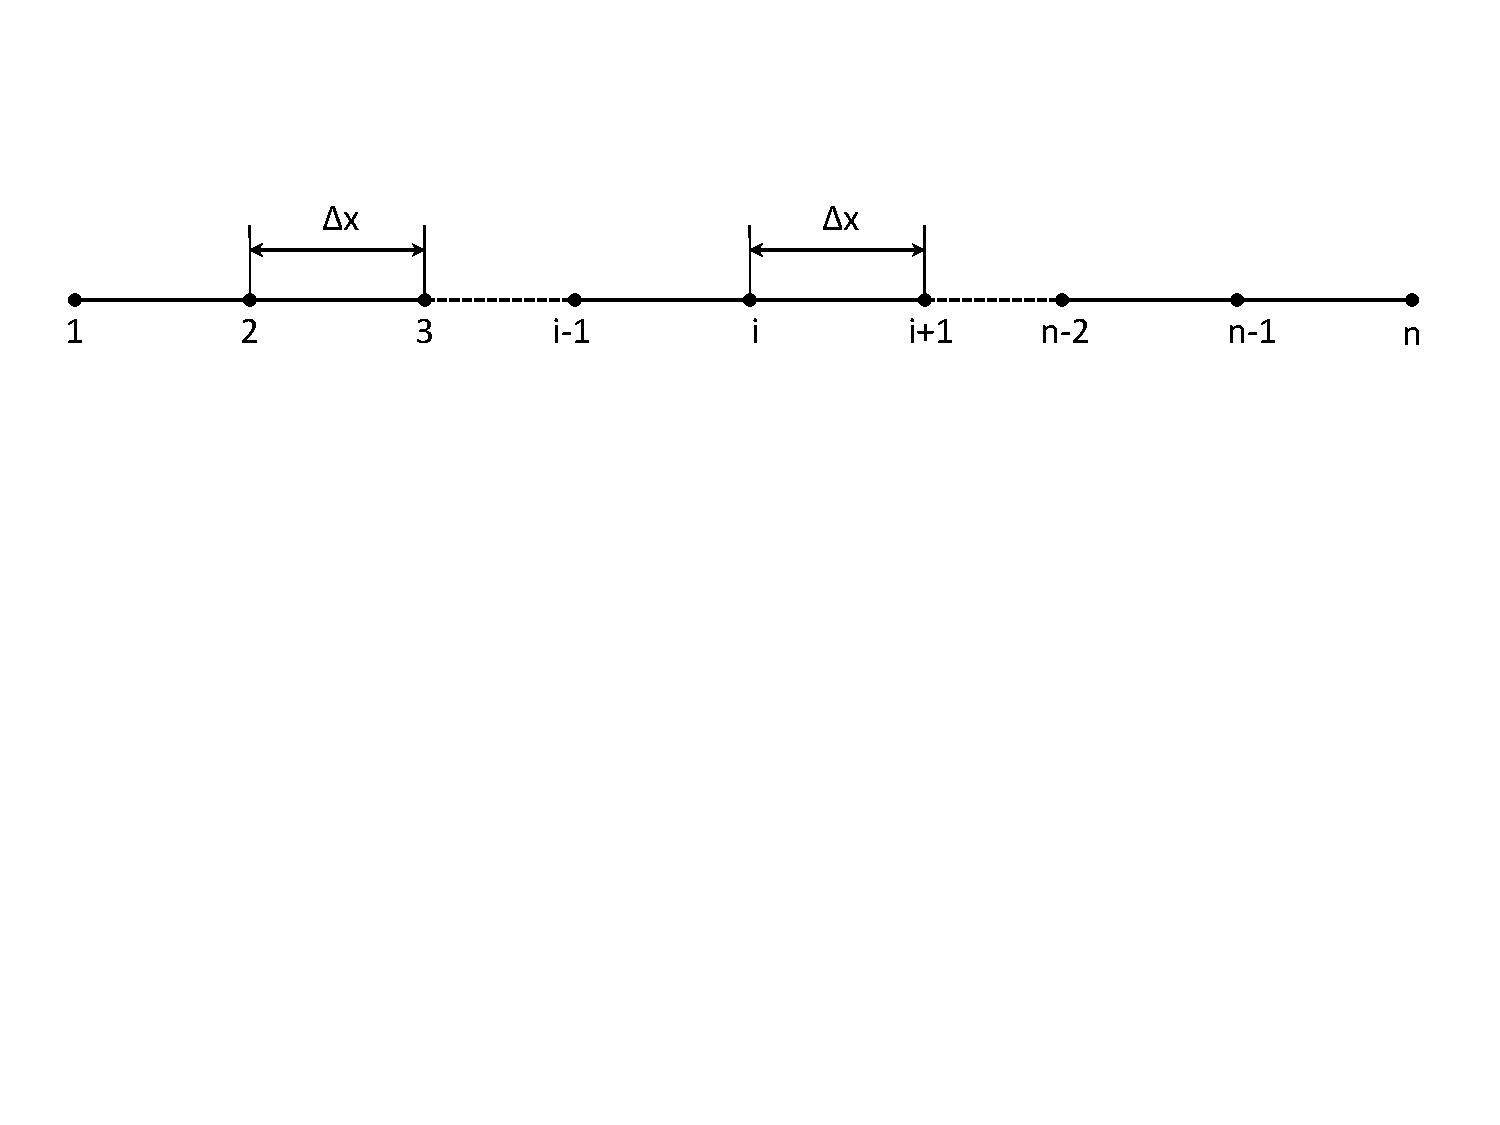
\includegraphics[width=11.5cm, height=1.5cm, clip]{./Pics/SchetchFDM.pdf}
       \end{center}}

\end{frame}


%%%
%%% Slide
%%% 
\begin{frame}
  \frametitle{Introduction to Finite Difference Methods (FDM)}
\begin{enumerate}
   \setcounter{enumi}{4}
  \item <1-> Thus, the diffusion term can be redefined as,
     \visible<1->{
     \begin{equation}
         \Gamma\left(\frac{d^{2}\phi}{dx^{2}}\right)_{2}=\Gamma\frac{\phi_{i-1}+\phi_{i+1}-2\phi_{i}}{\left(\Delta x\right)^{2}}\label{DiffusionEqn}
     \end{equation}}
  \item <2-> And the source term can be evaluated at point $i$, i.e., $\mathcal{S}_{i}=\mathcal{S}\left(\phi_{i}\right)$. Thus the discrete form of Eqn~\ref{eq:1Dtransport_simplified} is,
     \visible<2->{
     \begin{equation}
         \Gamma\frac{\partial^{2}\phi}{\partial x^{2}} +\mathcal{S} = \Gamma\frac{\phi_{i-1}+\phi_{i+1}-2\phi_{i}}{\left(\Delta x\right)^{2}} + \mathcal{S}\left(\phi_{i}\right)
     \end{equation} }
  \item <3-> Here, we have a system of algebraic equations (for each point of the mesh) that can determine discrete values for $\phi$;
  \item <4-> The resulting system of equations can be solved by any (direct or iterative) method;
  \item <5-> The FDM is not inherently conservative, and can only be used in relatively simple geometries as it relies on structured grids.
\end{enumerate}  
 
\end{frame}


%%%
%%% Slide
%%% 
\begin{frame}
  \frametitle{Solving 1D Transient HT Problems with FDM}
     \begin{columns}
        \begin{column}[c]{0.45\linewidth}
           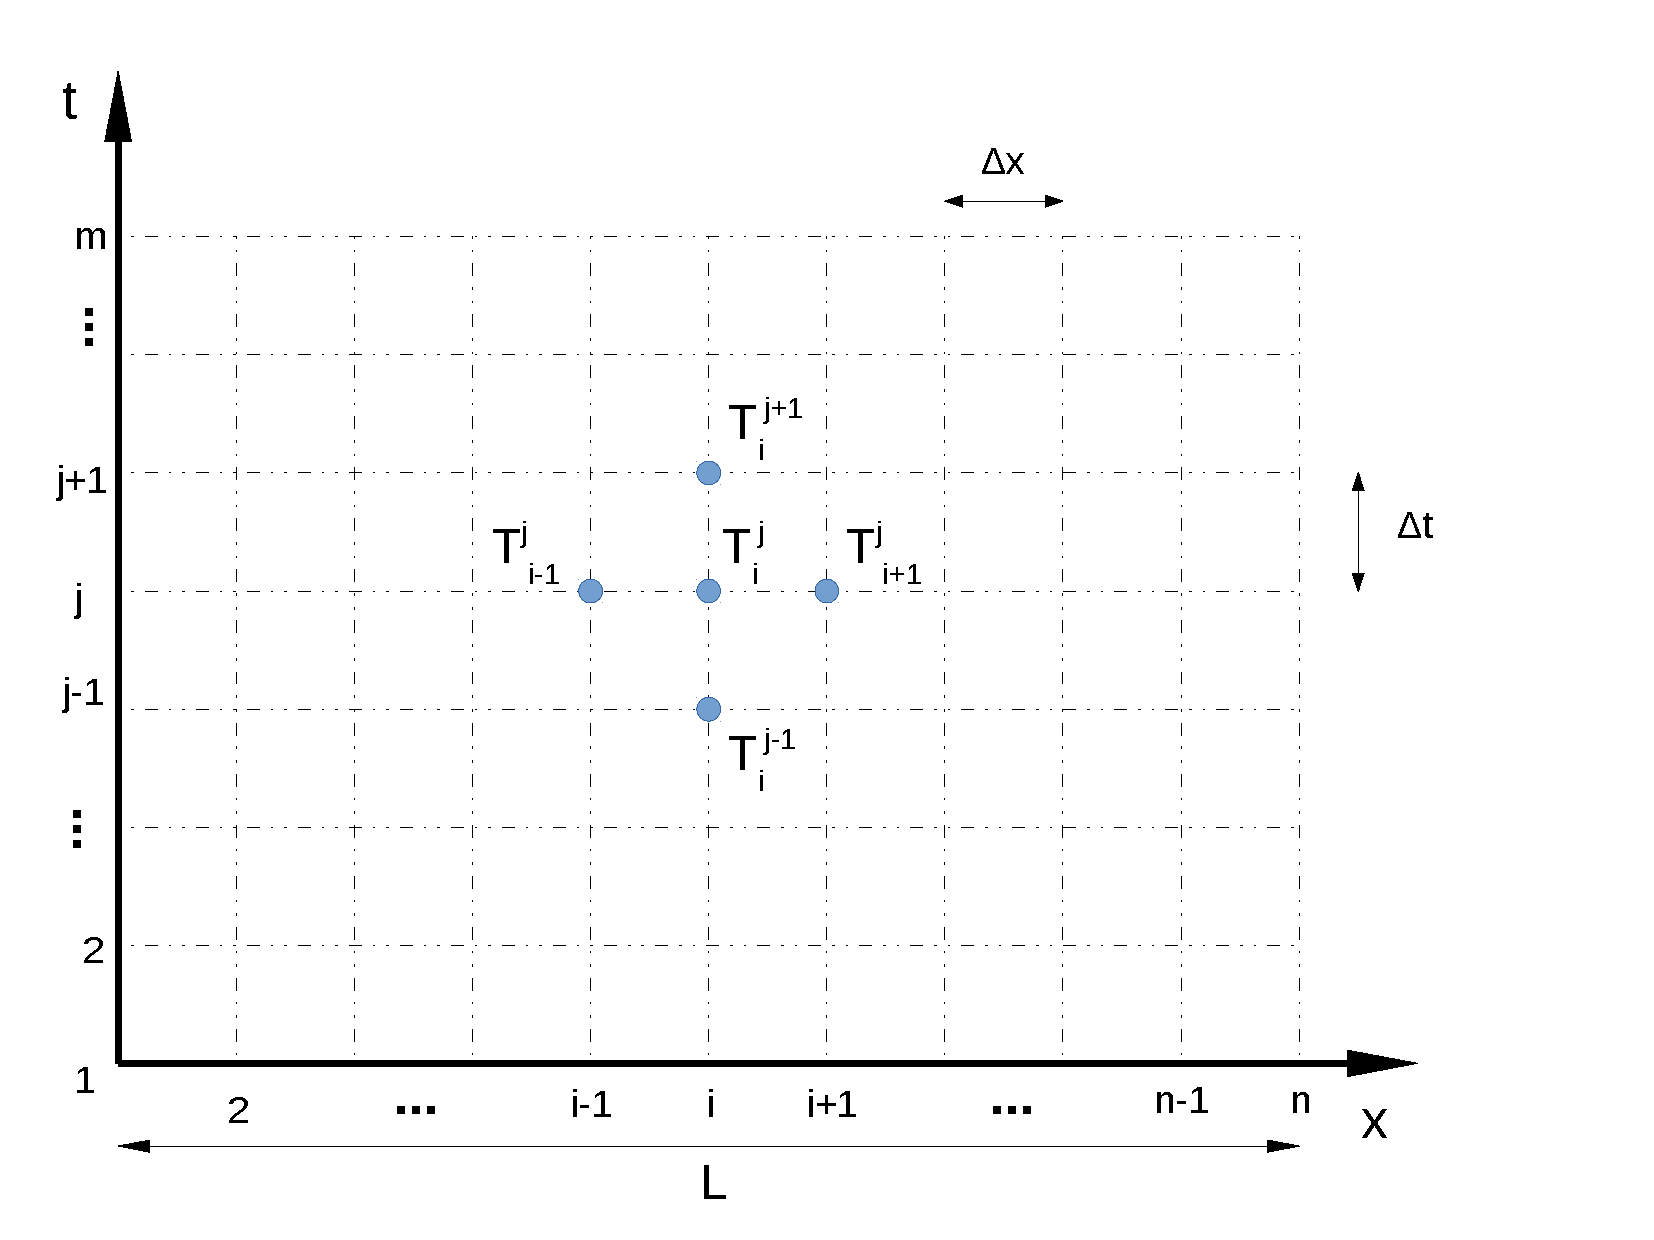
\includegraphics[width=1.2\columnwidth,height=1.3\columnwidth,clip]{./Pics/FDM_1DTransient}
        \end{column}
        \begin{column}[l]{0.55\linewidth}
           \begin{enumerate}
              \item<1-> The 1D transient heat conduction problem in a slab $L$ with constant properties is represented by Eqn.~\ref{Eqn:GlobalThermalEqn},
                  \visible<1->{\begin{displaymath}
                     \frc{\partial^{2} T}{\partial x^{2}} = \frc{1}{\alpha}\frc{\partial T}{\partial t}\label{Eqn:GlobalThermalEqn}
                  \end{displaymath}
                  subjected to prescribed \blue{boundary and initial conditions} for $T(x,t)$. }
              \item<2-> In FDM, the spatial- and time-domains are divided into mesh grid. The points in both coordinates are separated by constant spacing, $\Delta x$ and $\Delta t$;
              \item<2-> Nodes $x_{1}$ and $x_{n}$ are \blue{boundaries nodes} whereas all other nodes are \blue{interior nodes};
              \item<3-> Node $t_{1}$ represents the \blue{initial condition} of the system.
           \end{enumerate}
        \end{column}
     \end{columns}
\end{frame}


%%%
%%% Slide
%%%
\begin{frame}
  \frametitle{Solving 1D Transient HT Problems with FDM}
    \begin{enumerate}\setcounter{enumi}{4}
      \item<1-> The diffusion term, 
         \visible<1->{\begin{displaymath}
             \nabla\cdot\left(\alpha \nabla T\right) = \frc{\partial}{\partial x}\left(\alpha\frc{\partial T}{\partial x}\right) = \alpha\frc{\partial^{2} T}{\partial x^{2}}
         \end{displaymath}
         can be discretised in space (following Eqn.~\ref{DiffusionEqn}),}
         \visible<2->{\begin{equation}
            \alpha\frc{\partial^{2} T}{\partial x^{2}} = \alpha \frc{T_{i+1} - 2T_{i} + T_{i-1}}{\left(\Delta x\right)^{2}}\label{eqn:spatial_term}
         \end{equation}
         where $\Delta x = x_{i+1}-x_{i} = x(i+1)-x(i)$ and $T_{i}=T\left(x_{i}\right)$;}
      \item<3-> The time term, $\frc{\partial T}{\partial t}$ can be discretised using Taylor expansion (Eqn.~\ref{Eqn:FDMDisc2}) but truncated at lower order,
         \visible<3->{\begin{equation}
             \frc{\partial T}{\partial t} = \frc{T^{j+1}-T^{j}}{\Delta t}\label{eqn:time_term}
         \end{equation}
         where $\Delta t = t_{j+1}-t_{j}$ is the \blue{time-step size};}
    \end{enumerate}
\end{frame}

%%%
%%% Slide
%%%
\begin{frame}
  \frametitle{Solving 1D Transient HT Problems with FDM}
    \begin{enumerate}\setcounter{enumi}{6}
      \item<1-> Now substituting and arranging Eqns.~\ref{eqn:spatial_term}-~\ref{eqn:time_term} in Eqn.~\ref{DiffusionEqn}, with subscript $i$ and superscript $j$ representing spatial- and time-discretisation, respectively,
         \visible<1->{\begin{equation}
            T_{i}^{j+1} = T_{i}^{j} + \frc{\alpha\Delta t}{\left(\Delta x\right)^{2}}\left(T_{i+1}^{j}-2T_{i}^{j}+T_{i-1}^{j}\right)\label{ExplicitScheme}
         \end{equation}}
      \item<2-> The transient problem may be subject to \blue{boundary conditions} of the following types:
         \begin{enumerate}
            \item<2-> Dirichlet BC: 
                 \visible<2->{\begin{eqnarray}
                      && T\left(x=0,t_{j}\right) = T_{1}^{j} = \Psi_{1} \;\;\; \text{ and/or } \nonumber \\
                      && T\left(x=L,t_{j}\right) = T_{n}^{j} = \Psi_{2} \nonumber 
                 \end{eqnarray}
                 where $\Psi_{1}$ and $\Psi_{2}$ are either constants or functions;}
            \item<3-> Robin BC: prescribed flux, 
                \visible<3->{\begin{eqnarray}
                   &&-\kappa\frc{\partial}{\partial x}T\left(x_{n},t_{j}\right) = h\left[T\left(x_{n},t_{j}\right)-T_{\infty}\right] \text{or in indices notation,}\nonumber \\
                   &&-\kappa\frc{\partial T_{n}^{j}}{\partial x} = h\left(T_{n}^{j}-T_{\infty}\right) \nonumber
                \end{eqnarray}}
         \end{enumerate}

    \end{enumerate}
\end{frame}


%%%
%%% Slide
%%%
\begin{frame}
  \frametitle{Solving 1D Transient HT Problems with FDM}
    \begin{enumerate}\setcounter{enumi}{8}
      \item<1-> In Eqn.~\ref{ExplicitScheme}, the new temperature (i.e., at \blue{time-step} $t_{j+1}$) is obtained from the old temperature  (i.e., at \blue{time-step} $t_{j}$). This is known as \red{explicit method}; 
      \item<2-> The explicit method is easy to use, however it suffers from an undesirable feature that severely restricts its utility -- {\bf it is not unconditionally stable}, i.e., its use is restricted by the time-step size, $\Delta t$;
      \item<3-> If the time-step is not sufficiently small, the solutions obtained by the explicit method may oscillate and diverge from the actual solution;
      \item<4-> In order to avoid these numerical oscillations, $\Delta t$ must be kept below a certain upper limit established by the \blue{stability criterion}, based on the \red{Fourier number},
           \visible<4->{\begin{equation}
               Fo = \frc{\alpha \Delta t}{\left(\Delta x\right)^{2}} \leq \frc{1}{2}
           \end{equation}} 

    \end{enumerate}
\end{frame}



%%%
%%%  SECTION
%%%
\section{Summary} 


%%% Slide
%%%
\begin{frame}
  \frametitle{Summary}
    \begin{enumerate}  
       \item Lumped capacity methods;  
       \item Analytical methods using Heisler and Gr\"ober charts;
       \item Finite-difference methods for 1D heat conduction problems.
    \end{enumerate}
\end{frame}








%%%
%%% Appendix
%%%
\section{Appendices}

\subsection{Appendix 1: Coefficients and Bessel Functions}\label{appendix1}
%%%
%%% Slide
%%%
\begin{frame}
 \frametitle{Coefficients and Bessel Functions}
        \begin{center}
          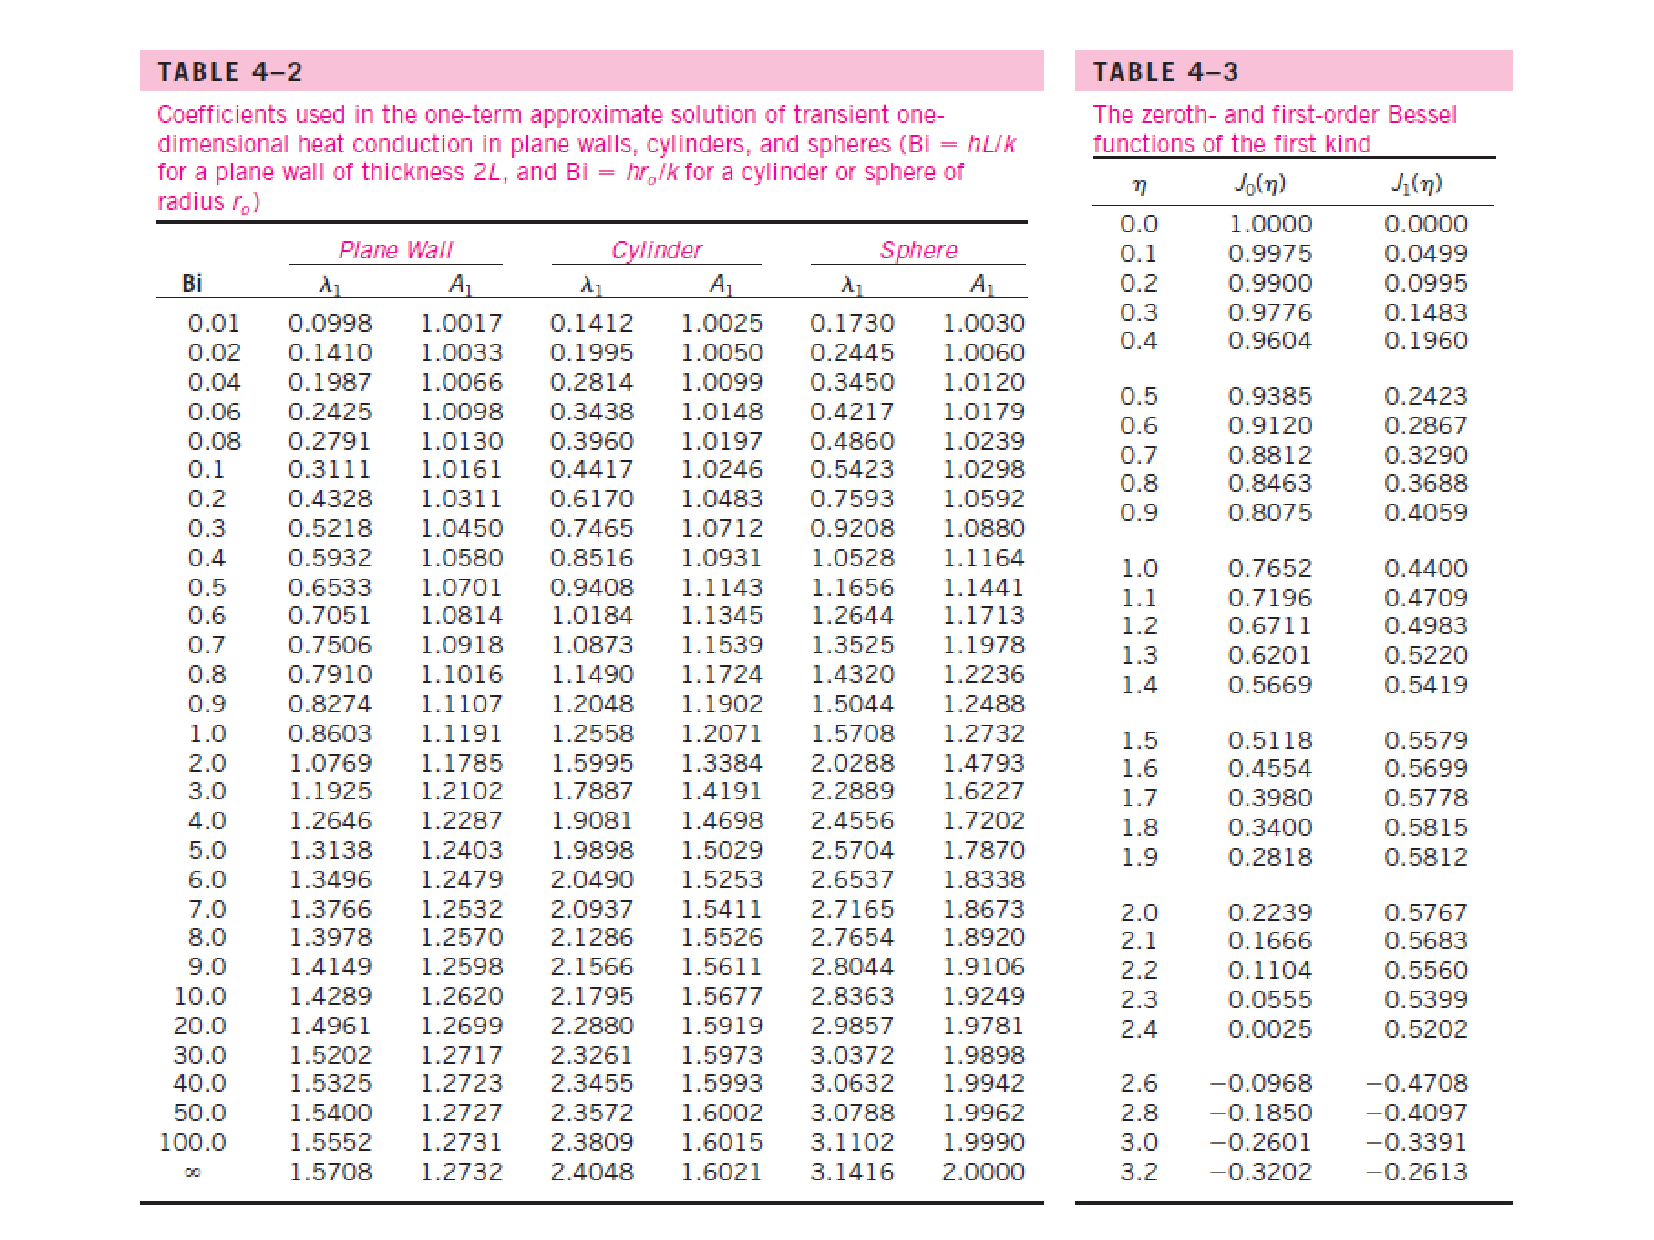
\includegraphics[width=.9\columnwidth,height=.65\columnwidth,clip]{./Pics/BaselFunctionTable}
        \end{center}
\end{frame}




\subsection{Appendix 2: Heisler and Gr\"ober Charts}\label{appendix2}
{
  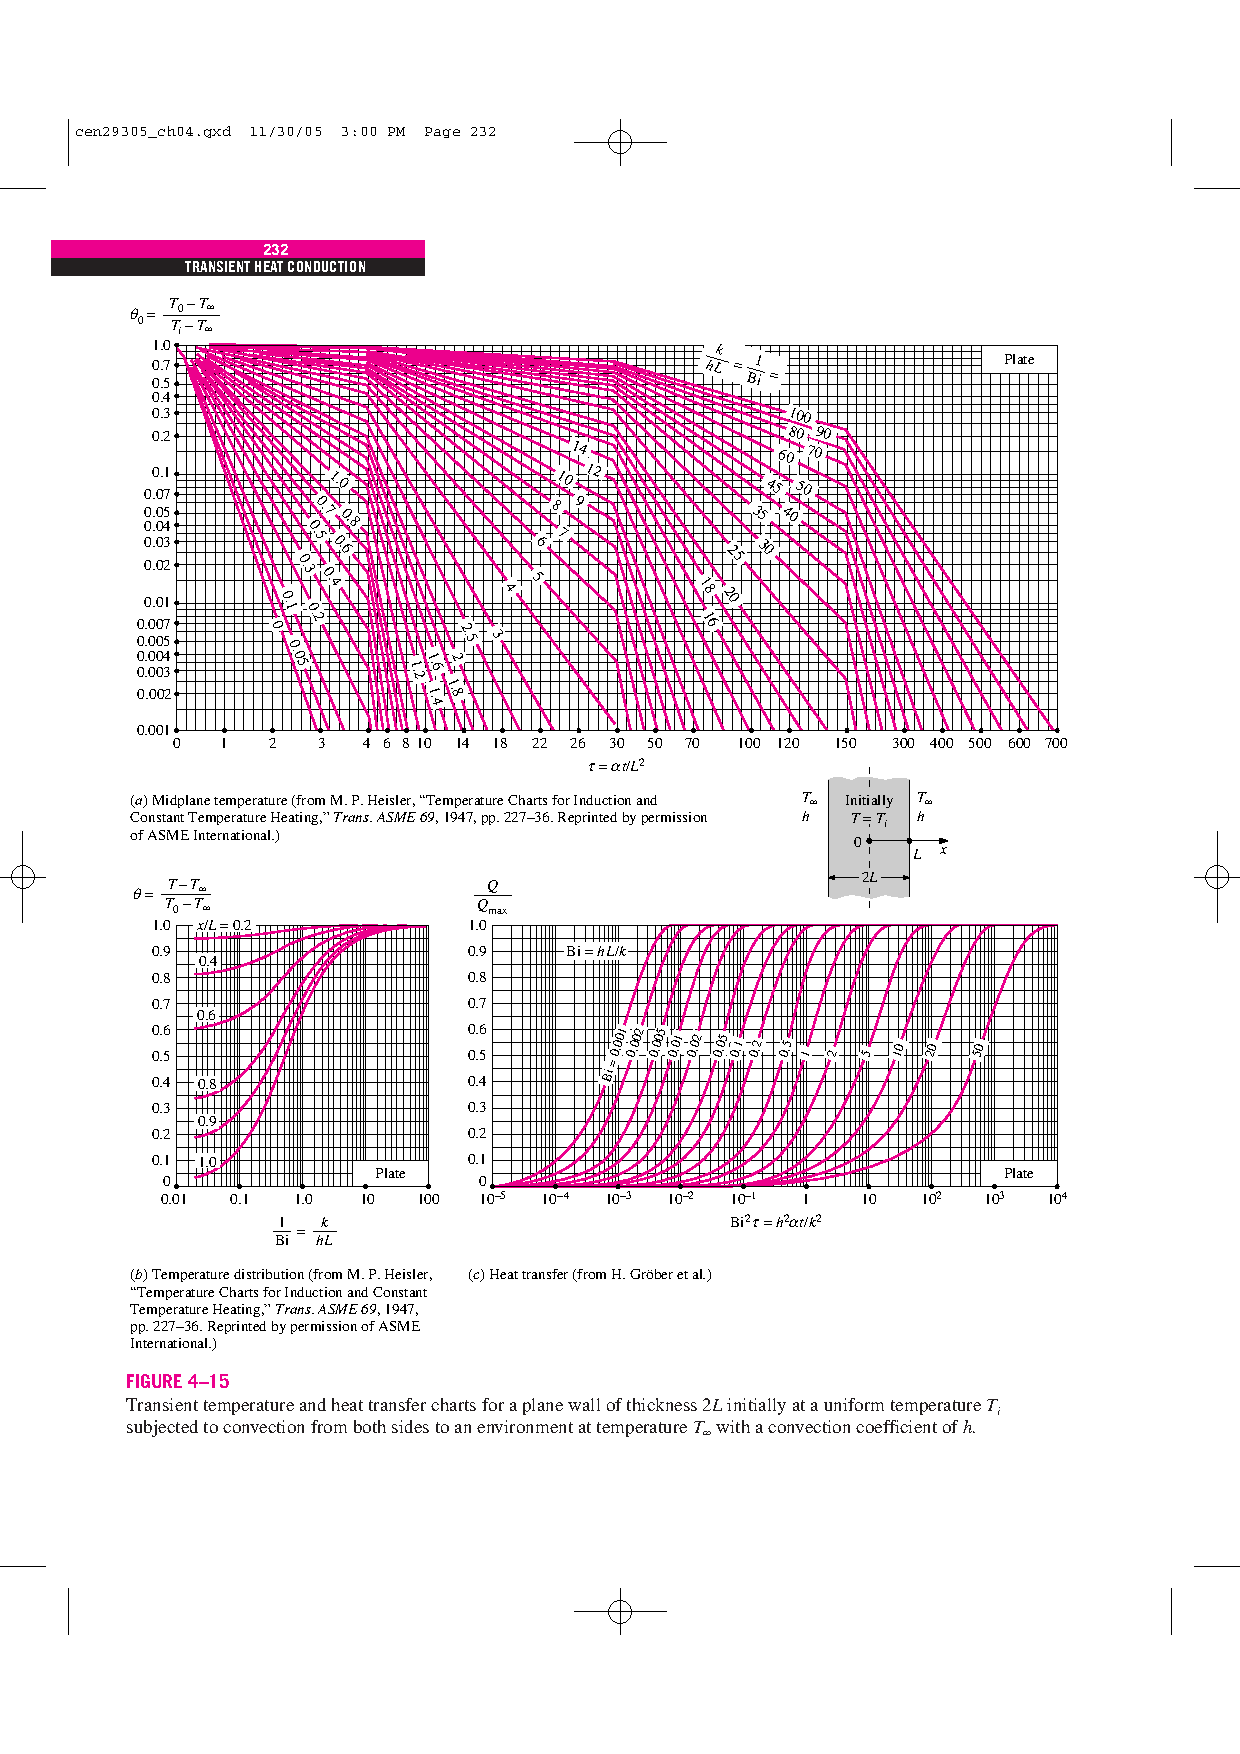
\includepdf[pages=-,fitpaper]{./Pics/HeislerCharts_All.pdf}
}


\end{document}
